% Dieser Text ist urheberrechtlich gesch�tzt
% Er stellt einen Auszug eines von mir erstellten Referates dar
% und darf nicht gewerblich genutzt werden
% die private bzw. Studiums bezogen Nutzung ist frei
% Mai. 2007
% Autor: Sascha Frank 
% Universit�t Freiburg 
% www.informatik.uni-freiburg.de/~frank/
\documentclass{beamer}
% \documentclass[notes=only]{beamer}
\usepackage{pst-bar,pst-plot,pstricks-add}
\usepackage{graphics,graphicx}
\usepackage{pstricks,pst-node,pst-tree}
% \setbeameroption{show notes}
\setcounter{tocdepth}{1}

\setbeamertemplate{navigation symbols}{}
\beamersetuncovermixins{\opaqueness<1>{25}}{\opaqueness<2->{15}}
\usetheme{CambridgeUS}
\usecolortheme{seahorse}

\begin{document}
	\title{The max-min-hill-climbing algorithm}  
	\author[M. Bauer]{Michael Bauer}
	\institute[M.Sc. Comp. Science]{M.Sc. Comp. Science}
	\date{\today}


\begin{frame}
	\titlepage
\end{frame}

\section{$\bar{MMPC}$}
	\begin{center}
		\begin{frame}
			\begin{center}
				\begin{figure}
					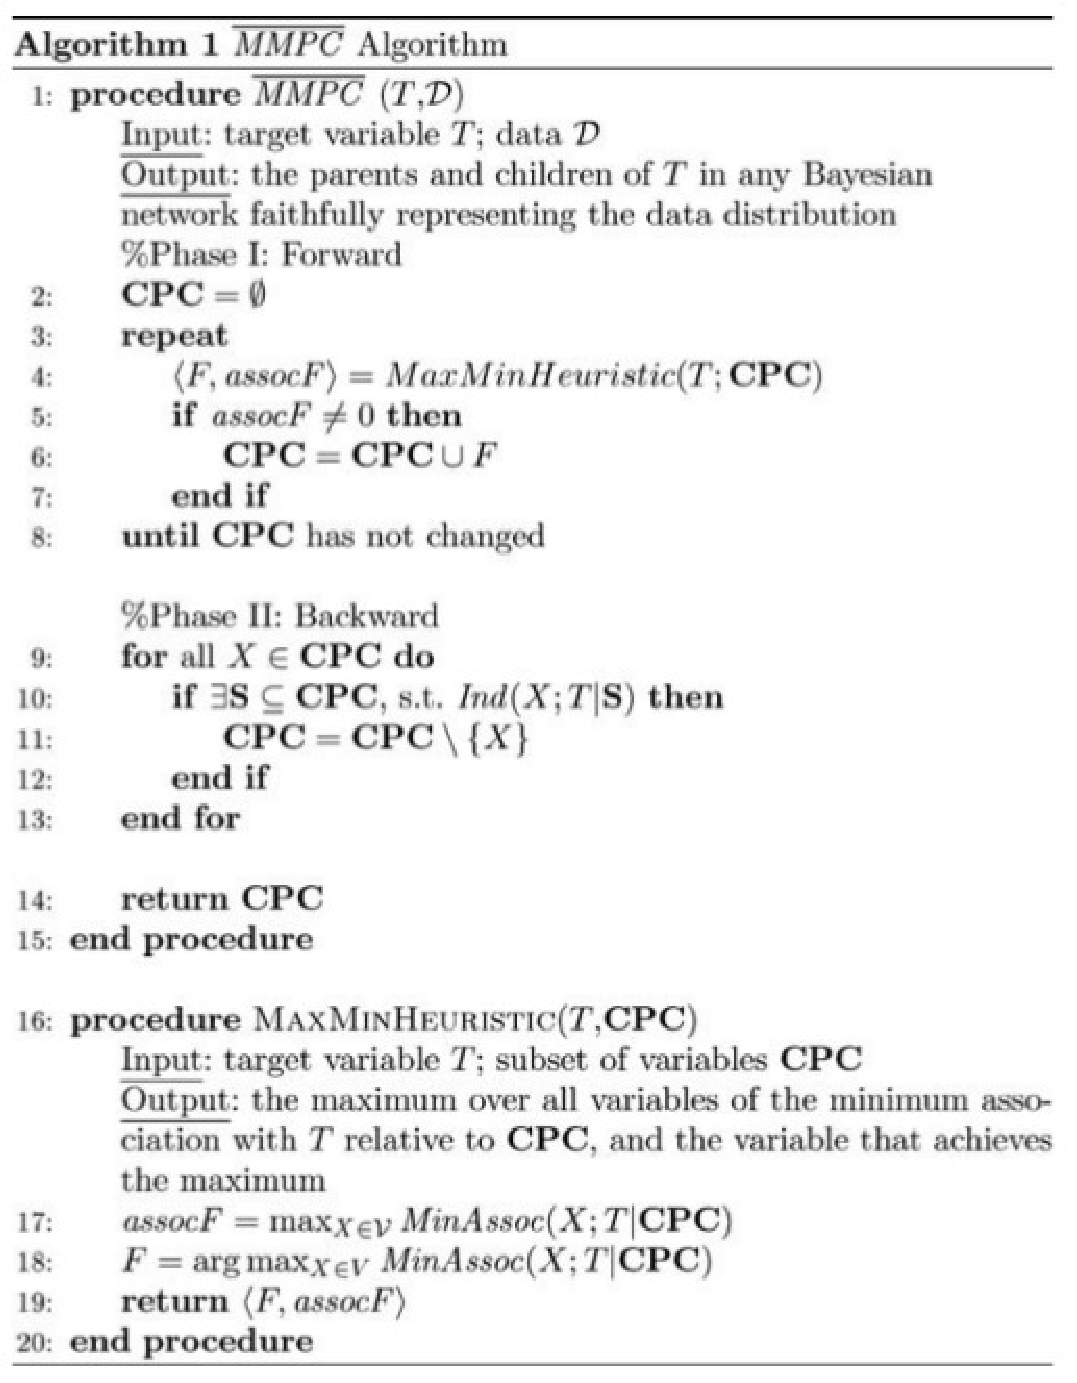
\includegraphics[scale=0.3]{img/mmpc_bar}
				\end{figure}
			\end{center}
		\end{frame}
	\end{center}

\section{Statistics}
	\subsection{The $G^{2}$ value}
		\begin{frame}
			\begin{block}{Definition}
				We calculate the $G^{2}$ value under the nullhypothesis of the conditional independence of $Ind_{P}(X_{i},X_{j}|\textbf{X}_{k})$ holding. Then, the $G^{2}$ value is defined as:
				\begin{equation}
					G^{2} := 2 * \sum_{a,b,c} S^{ab\textbf{c}}_{ijk} * ln \left( \frac{S^{ab\textbf{c}}_{ijk}*S^{\textbf{c}}_{k}}{S^{a\textbf{c}}_{ik}*S^{b\textbf{c}}_{jk}} \right),
				\end{equation}
				where $S^{abc}$ is the number of times in the data where $X_{i} = a$, $X_{j} = b$ and $\textbf{X}_{k} = \textbf{c}$. We define in a similar fashion $S^{ac}$, $S^{bc}$ and $S^{c}$, respectively. 

			\end{block}
		\end{frame}

	\subsection{Query the graph}
		\begin{center}
		\begin{frame}
			\begin{center}
				\begin{figure}
					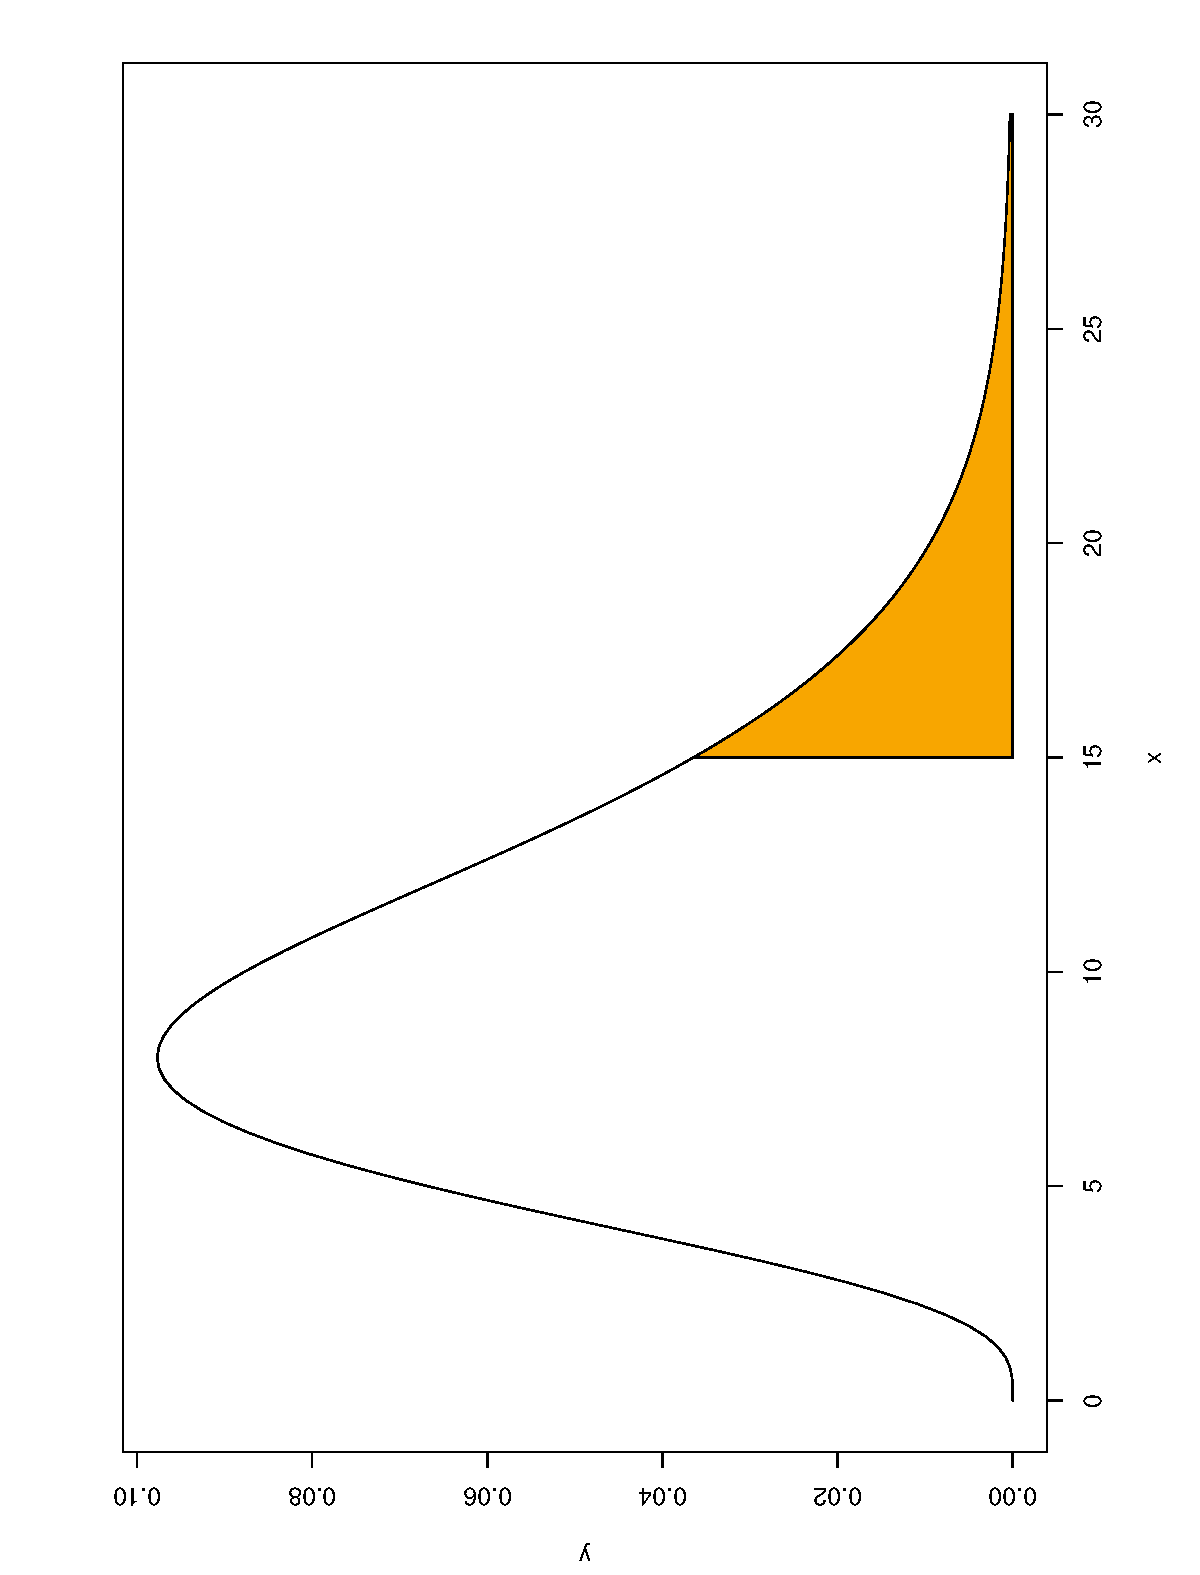
\includegraphics[scale=0.3, angle = 270]{img/chi}
				\end{figure}
			\end{center}
		\end{frame}
	\end{center}

\section{MMPC}
	\begin{center}
		\begin{frame}
			\begin{center}
				\begin{figure}
					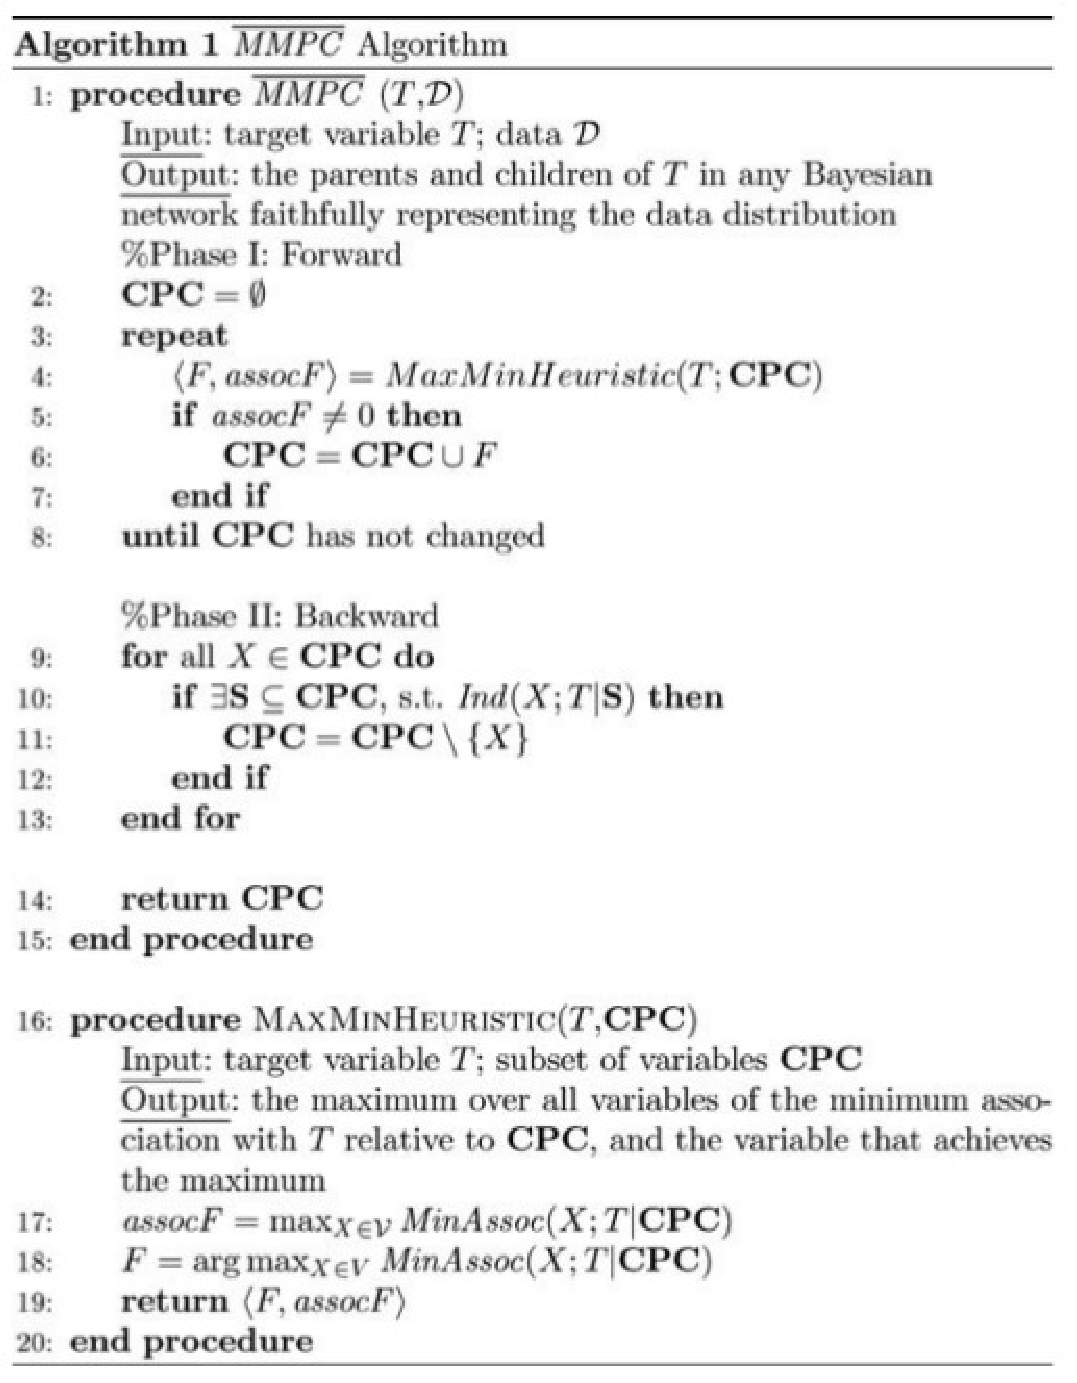
\includegraphics[scale=0.4]{img/mmpc_bar}
				\end{figure}
			\end{center}
		\end{frame}
	\end{center}

\section{Backward phase}
	\begin{center}
		\begin{frame}
			\begin{center}
				\begin{figure}
					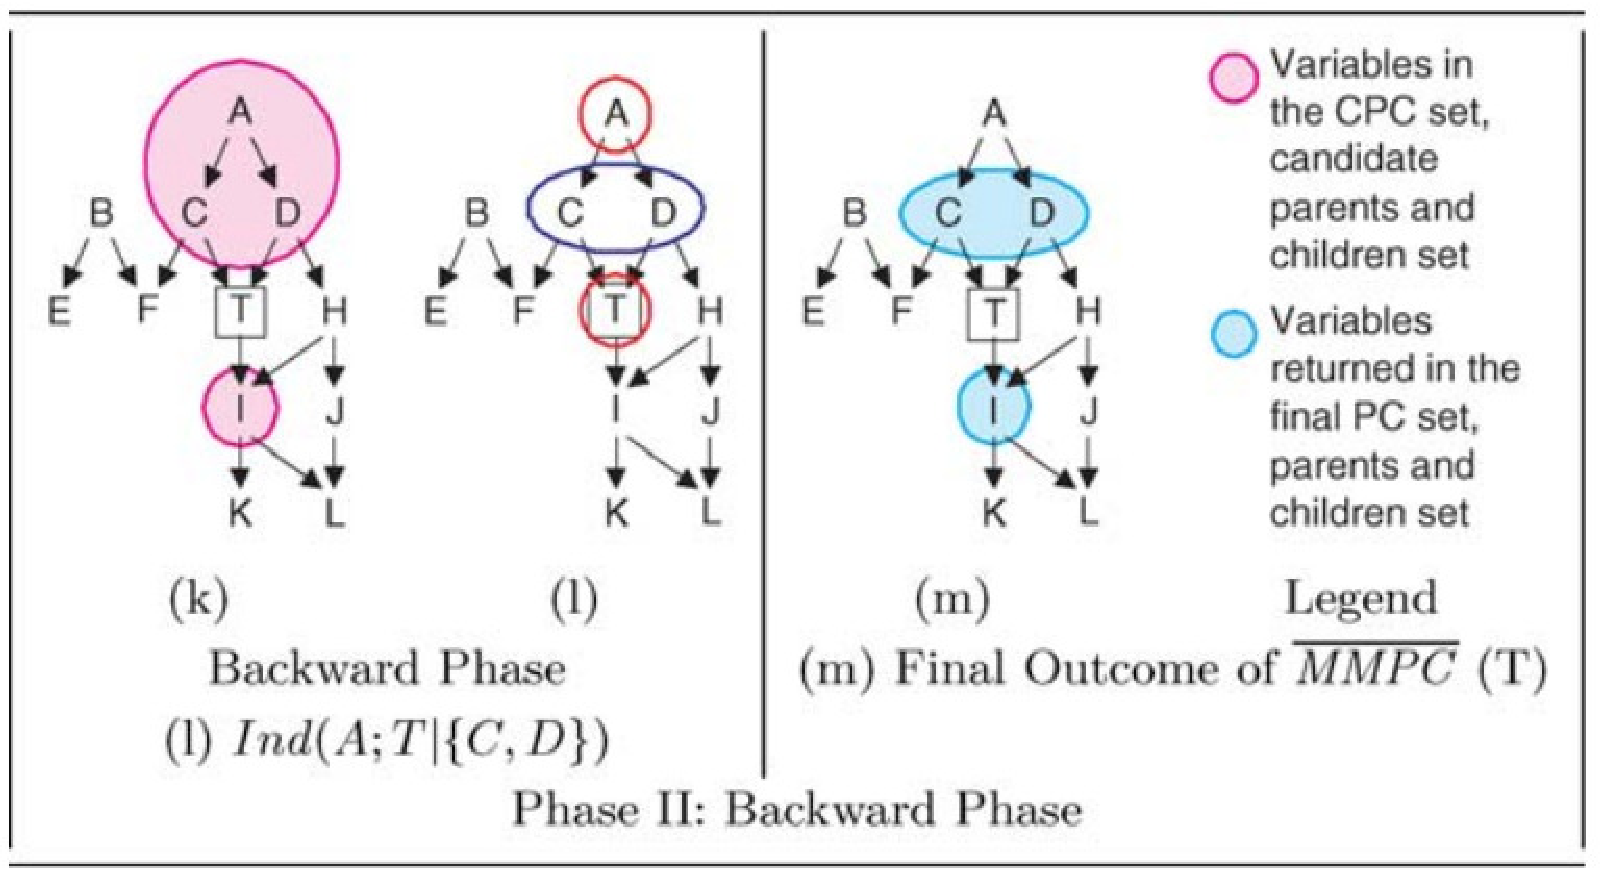
\includegraphics[scale=0.3]{img/backward}
				\end{figure}
			\end{center}
		\end{frame}
	\end{center}

\section{MMPC}
	\begin{center}
		\begin{frame}
			\begin{center}
				\begin{figure}
					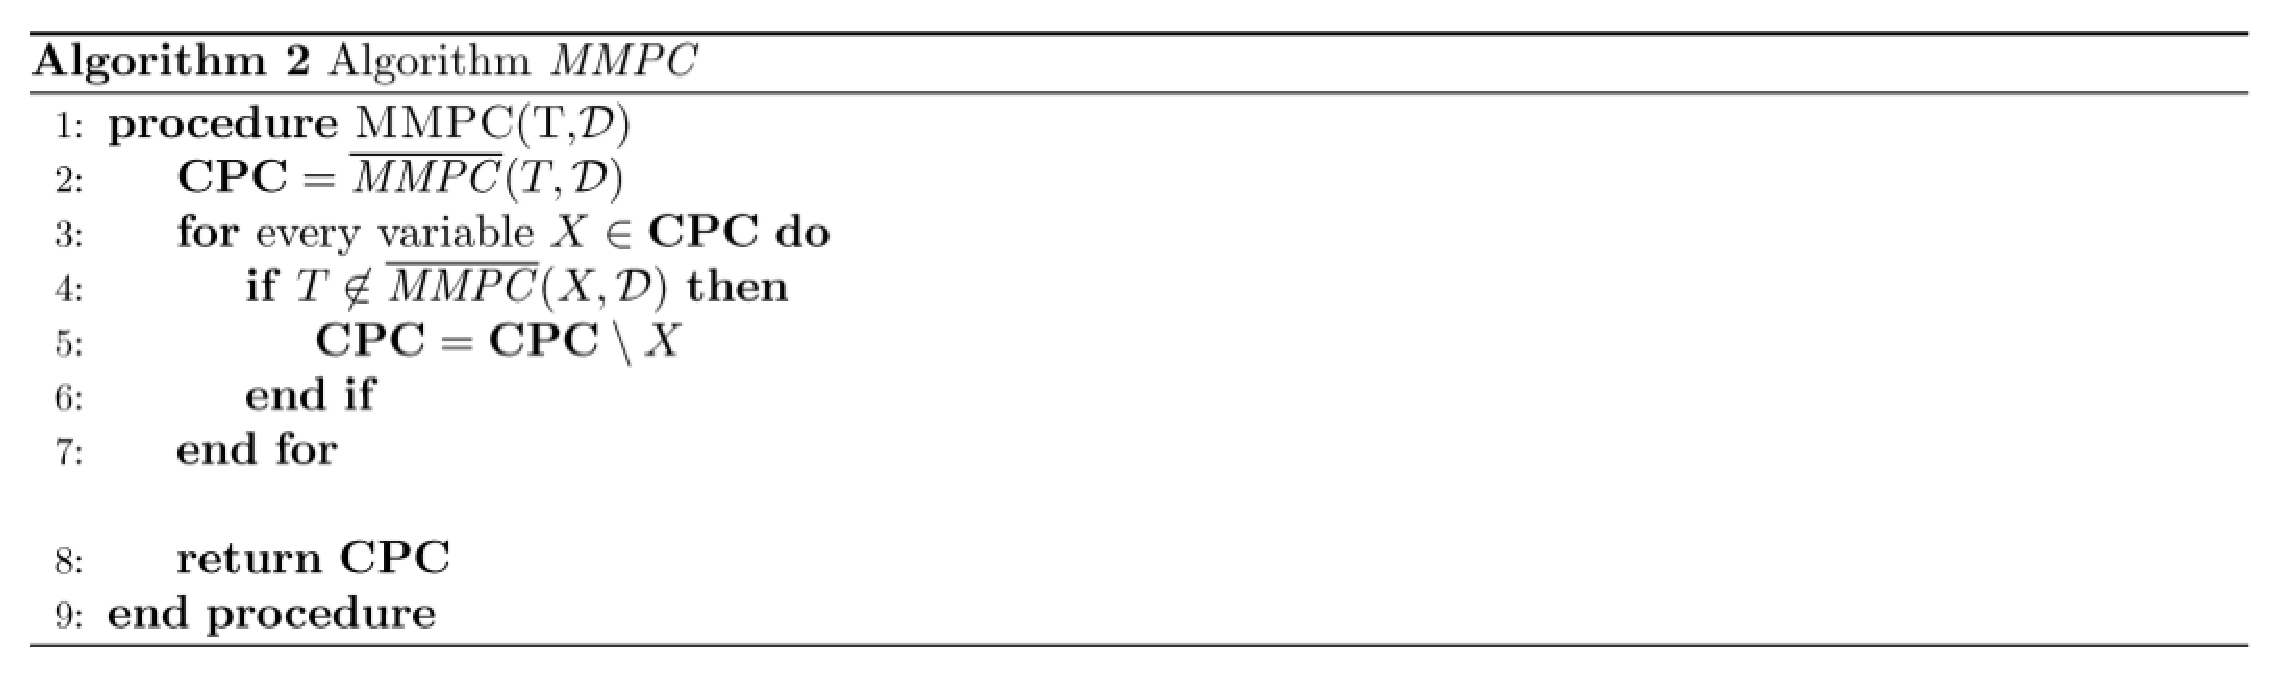
\includegraphics[scale=0.3]{img/mmpc}
				\end{figure}
			\end{center}
		\end{frame}
	\end{center}

\section{But...}
	\begin{center}
		\begin{frame}
			\begin{center}
				\begin{figure}
					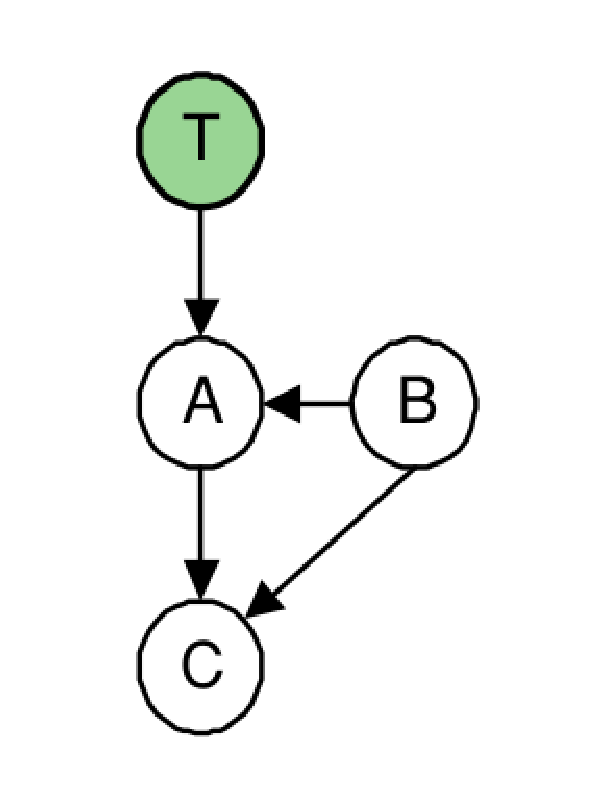
\includegraphics[scale=0.3]{img/falsePositive}
				\end{figure}
			\end{center}
		\end{frame}
	\end{center}

\section{Example}
	\begin{frame}
		\begin{small}
			\begin{psmatrix}[emnode=r,colsep=0.5cm,rowsep=0.6cm,mnodesize=2cm]
				[name=Tdiff]
					\begin{tabular}{|c|c|}
						\hline
						$\textbf{d}^{0}$ & $\textbf{d}^{1}$ \\
						\hline	0.6 & 0.4  \\
						\hline
						\end{tabular}
				&[name=Diff,mnode=circle]
					Difficulty
				&
				&[name=Intell,mnode=circle]
					Intelligence
				&[name=TInt]
					\begin{tabular}{|c|c|}
						\hline
						$\textbf{i}^{0}$ & $\textbf{i}^{1}$ \\
						\hline 0.7 & 0.3  \\
						\hline 
					\end{tabular}
				\\
				[name=TGrade]
					\begin{tabular}{|c|c|c|c|}
						\hline
						& $\textbf{g}^{1}$ & $\textbf{g}^{2}$ & $\textbf{g}^{3}$ \\
						\hline
						$\textbf{i}^{0}$,$\textbf{d}^{0}$ & 0.3 & 0.4 & 0.3  \\
						\hline
						$\textbf{i}^{0}$,$\textbf{d}^{1}$ & 0.05 & 0.25 & 0.7  \\
						\hline
						$\textbf{i}^{1}$,$\textbf{d}^{0}$ & 0.9 & 0.08 & 0.02  \\
						\hline
						$\textbf{i}^{1}$,$\textbf{d}^{1}$ & 0.5 & 0.3 & 0.2  \\
						\hline
					\end{tabular}
				&
				&[name=Grade,mnode=circle]Grade
				&
				&[name=SAT,mnode=circle]SAT
				\\
				[name=Tlet]
					\begin{tabular}{|c|c|c|}
						\hline
						& $\textbf{l}^{0}$ & $\textbf{l}^{1}$ \\
						\hline
						$\textbf{g}^{1}$ & 0.95 & 0.05  \\
						\hline
						$\textbf{g}^{2}$ & 0.2 & 0.8  \\
						\hline
						$\textbf{g}^{3}$ & 0.2 & 0.8  \\
						\hline
					\end{tabular}
				&
				&[name=Let,mnode=circle]Letter
				&[name=TSAT]
					\begin{tabular}{|c|c|c|}
						\hline
						& $\textbf{s}^{0}$ & $\textbf{s}^{1}$ \\
						\hline
						$\textbf{i}^{0}$ & 0.95 & 0.05  \\
						\hline
						$\textbf{i}^{1}$ & 0.2 & 0.8  \\
						\hline
					\end{tabular}
				&		
			\end{psmatrix}
		\end{small}
			\psset{nodesep=1pt,arrows=->}
			\ncline{Diff}{Grade}
			\ncline{Intell}{Grade}
			\ncline{Intell}{SAT}
			\ncline{Grade}{Let}
			\psset{nodesep=6pt,arrows=-}
			\ncline{Tdiff}{Diff}
			\ncline{TInt}{Intell}
			\ncline{TSAT}{SAT}
			\ncline{TGrade}{Grade}
			\ncline{Tlet}{Let}
	\end{frame}

\section{What's next?}
	\begin{center}
		\begin{frame}
			\begin{center}
				\begin{huge}
					Coming up soon: direct the edges
				\end{huge}
			\end{center}
		\end{frame}
	\end{center}

\section{Thank you!}
	\begin{frame}
		\begin{block}{\center{\Huge{Thanks for your attention!}}}\end{block}
	\end{frame}

% \section{The algorithm}
% 	\subsection{How the algorithm works}
% 		\begin{center}
% 			\begin{frame}
% 				\begin{center}
% 					\begin{figure}
% 						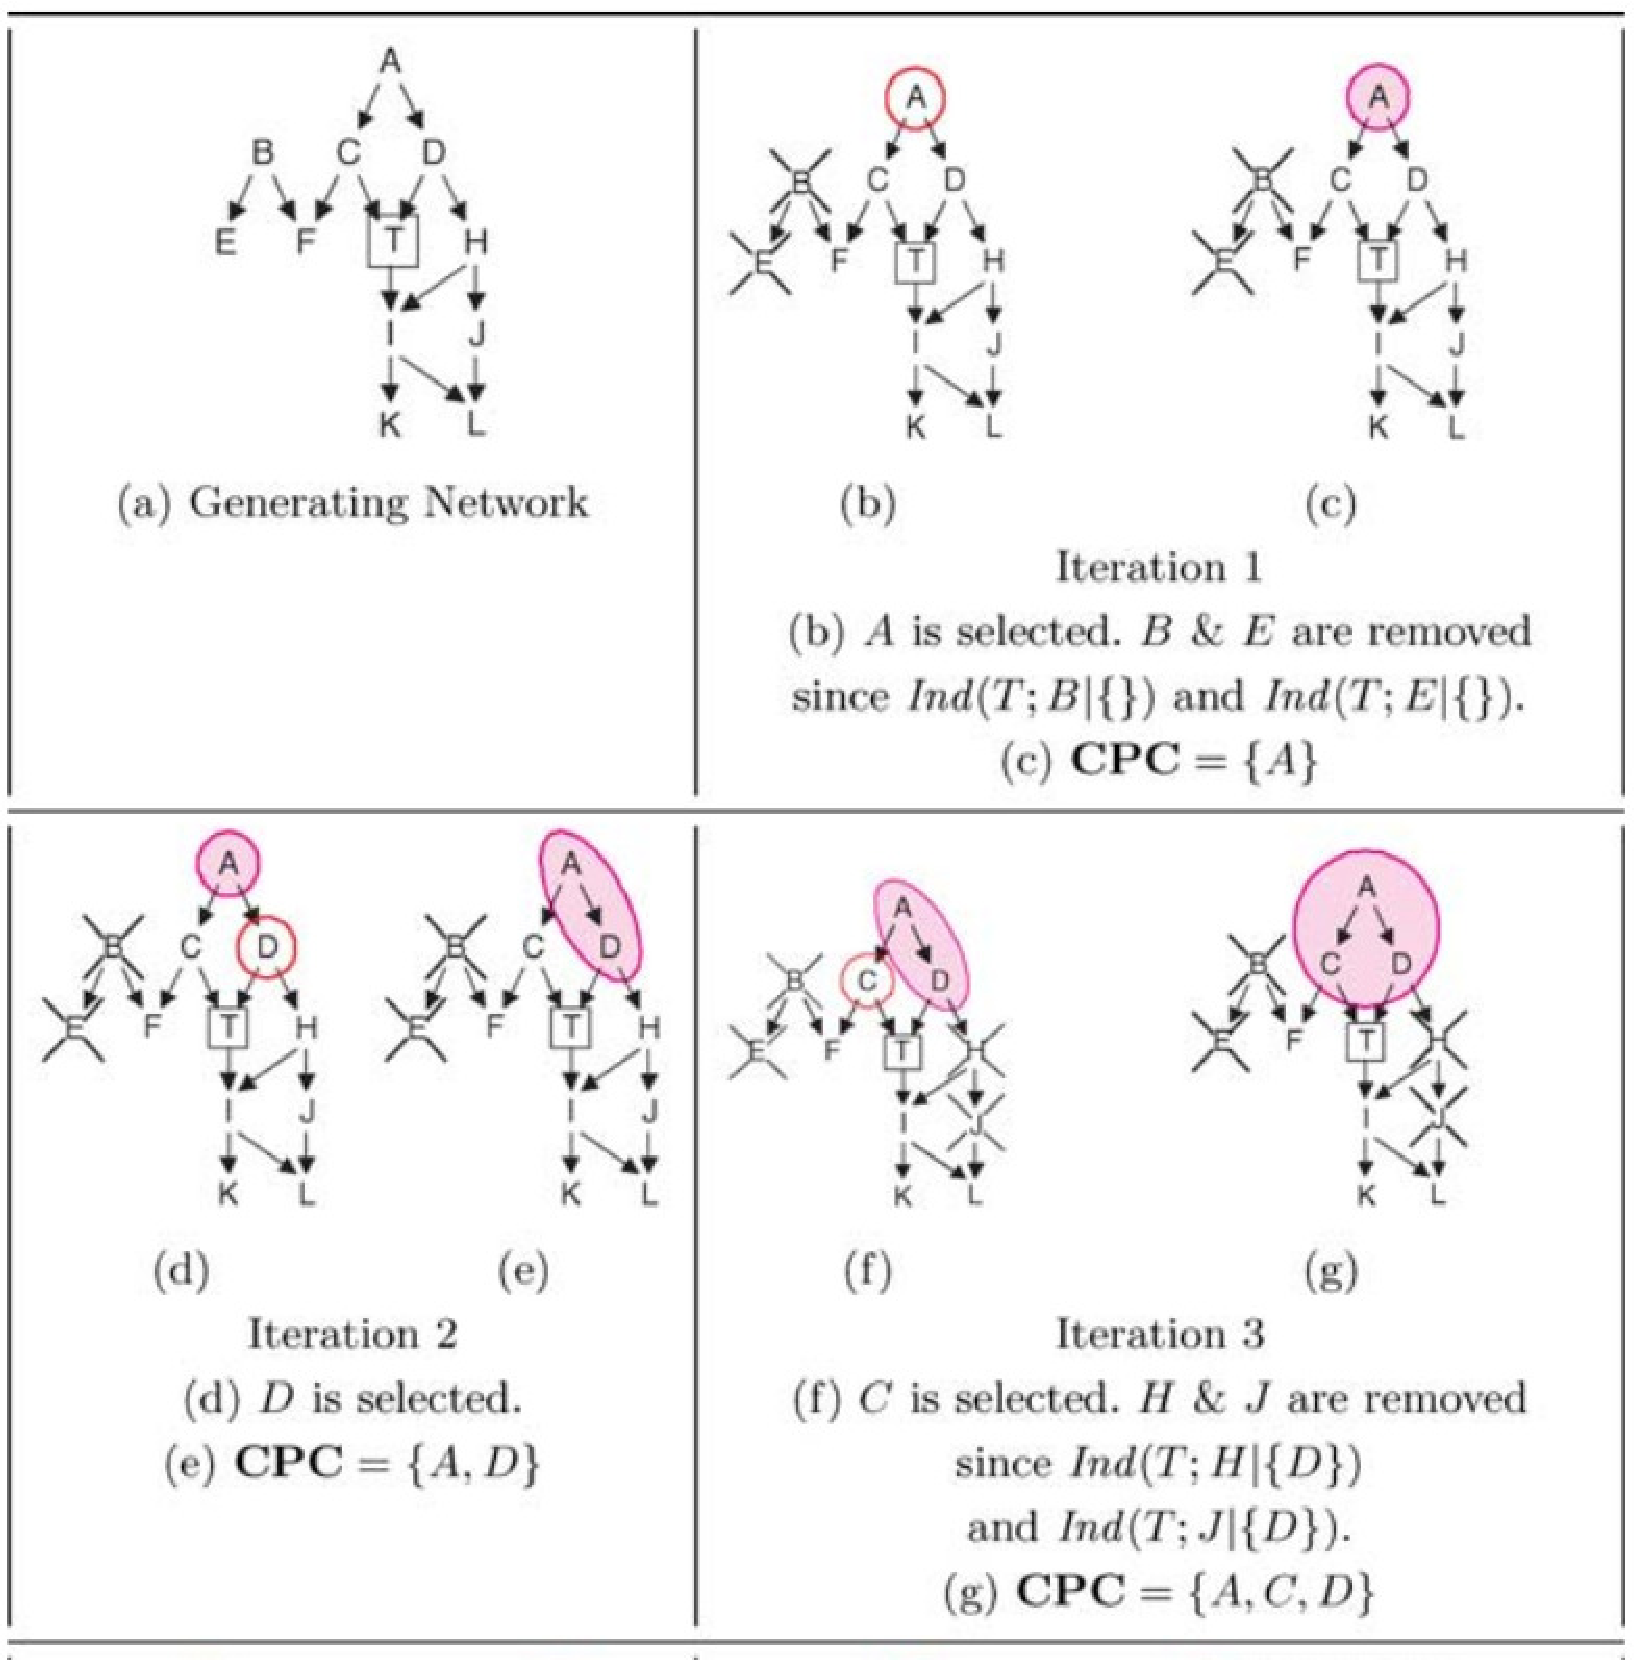
\includegraphics[scale=0.3]{img/example_part1}
% 					\end{figure}
% 				\end{center}
% 			\end{frame}
% 		\end{center}

% 	\subsection{How the algorithm works}
% 		\begin{center}
% 			\begin{frame}
% 				\begin{center}
% 					\begin{figure}
% 						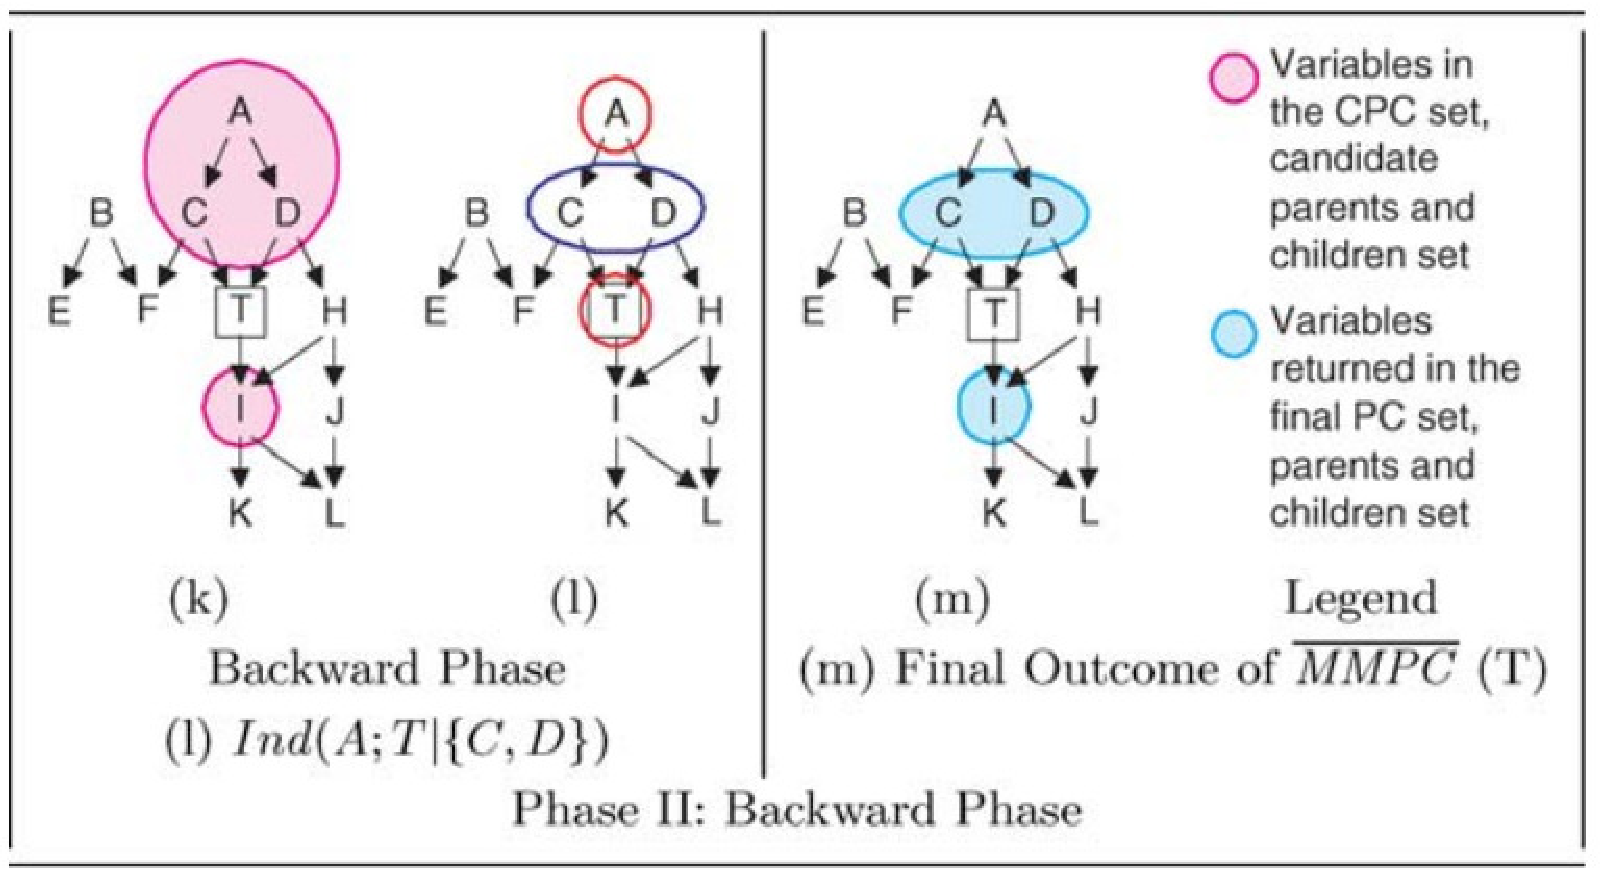
\includegraphics[scale=0.4]{img/example_part2}
% 					\end{figure}
% 				\end{center}
% 			\end{frame}
% 		\end{center}

\end{document}